Es un punto máximo que alcanza una onda al desplazarse. El punto más alto, donde la amplitud es máxima.

Es el punto más alejado de la posición de equilibrio en la dirección positiva del desplazamiento.

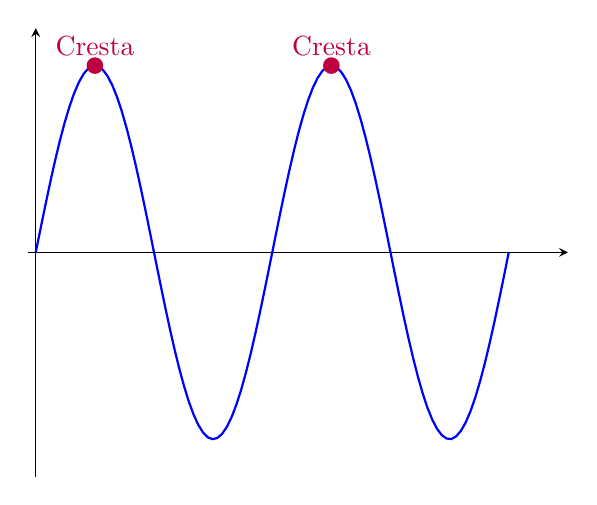
\begin{tikzpicture}
  \begin{axis}[
    xmin=-0.2,xmax=4.5*pi,
    ymin=-1.2,ymax=1.2,
    axis lines=middle,
    xtick={0},
    ytick={0}
    ]

    % Funcion senoidal
    \addplot[color=blue,samples=100,domain=0:4*pi,thick]{sin(deg(x))};

    % Cresta 1
    \fill[purple] (axis cs:pi/2,1) circle[radius=3pt];
    \node[purple,above] at (axis cs:pi/2,1) {Cresta};

    % Cresta 2
    \fill[purple] (axis cs:5*pi/2,1) circle[radius=3pt];
    \node[purple,above] at (axis cs:5*pi/2,1) {Cresta};
  \end{axis}
\end{tikzpicture}
